\documentclass[a4papper, 10pt]{article}

 \usepackage[utf8]{inputenc}
 \usepackage[T1]{fontenc}
 \usepackage[normalem]{ulem}
 \usepackage[french]{babel}
 \usepackage{graphicx}
 \usepackage{caption}
 \usepackage{subcaption}
 \usepackage{enumerate}
 \usepackage{array}
 \usepackage{amsmath,amssymb,mathrsfs}
 \usepackage{url}
 \usepackage{fullpage}
 \usepackage{todonotes}
 
 \title{\textbf{Intelligent detection layers for advanced tracking in high-energy physics} \\ \large \vskip 1ex
        Résumé de la thèse de doctorat}
\author{Benjamin Boitrelle \\ 
        Sous la direction de : \\
        Jérôme Baudot : Directeur de thèse à l'Université de Strasbourg \\
        Ingrid Maria Gregor : Encadrante au laboratoire d'accueil au DESY de Hambourg}
 \date{}

 \begin{document}

    \maketitle

% Questions posées : Flavor-tagging ILC, rapport embranchement du Higgs
% Méthode : montrer analyse Higgs avec résultats rapport d'embranchement
%           discuter 
% Résultats

  \section{Contexte de la thèse}

  Le 4 juillet 2012 au CERN à Genève (Suisse), les collaborations ATLAS et CMS ont annoncé les premiers résultats d'analyse des données acquises grâce au plus grand accélérateur de particules du monde, le Large Hadron Collider (LHC)\cite{Aad2012}\cite{Chatrchyan2012}. 
  Les deux expériences ont présenté la découverte de la signature d'une particule compatible avec le boson prédit par le mécanisme de la brisure de la symétrie électro-faible de Brout-Englert-Higgs, le boson de Higgs.
  Bien que l'augmentation de l'énergie de collision du LHC pourrait permettre une meilleure compréhension de cette nouvelle particule et de contraindre encore plus les limites du Modèle Standard, voire de découvrir des traces de physique au delà de cette théorie, la complexité des évènements générés limite l'accès à certains paramètres fondamentaux.
  %En effet, les protons sont des particules composites, c'est-à-dire constituées d'un assemblage de particules, dont leur structure cache les paramètres fondamentaux de la collision
  
  \begin{figure}[!h]
    \centering
    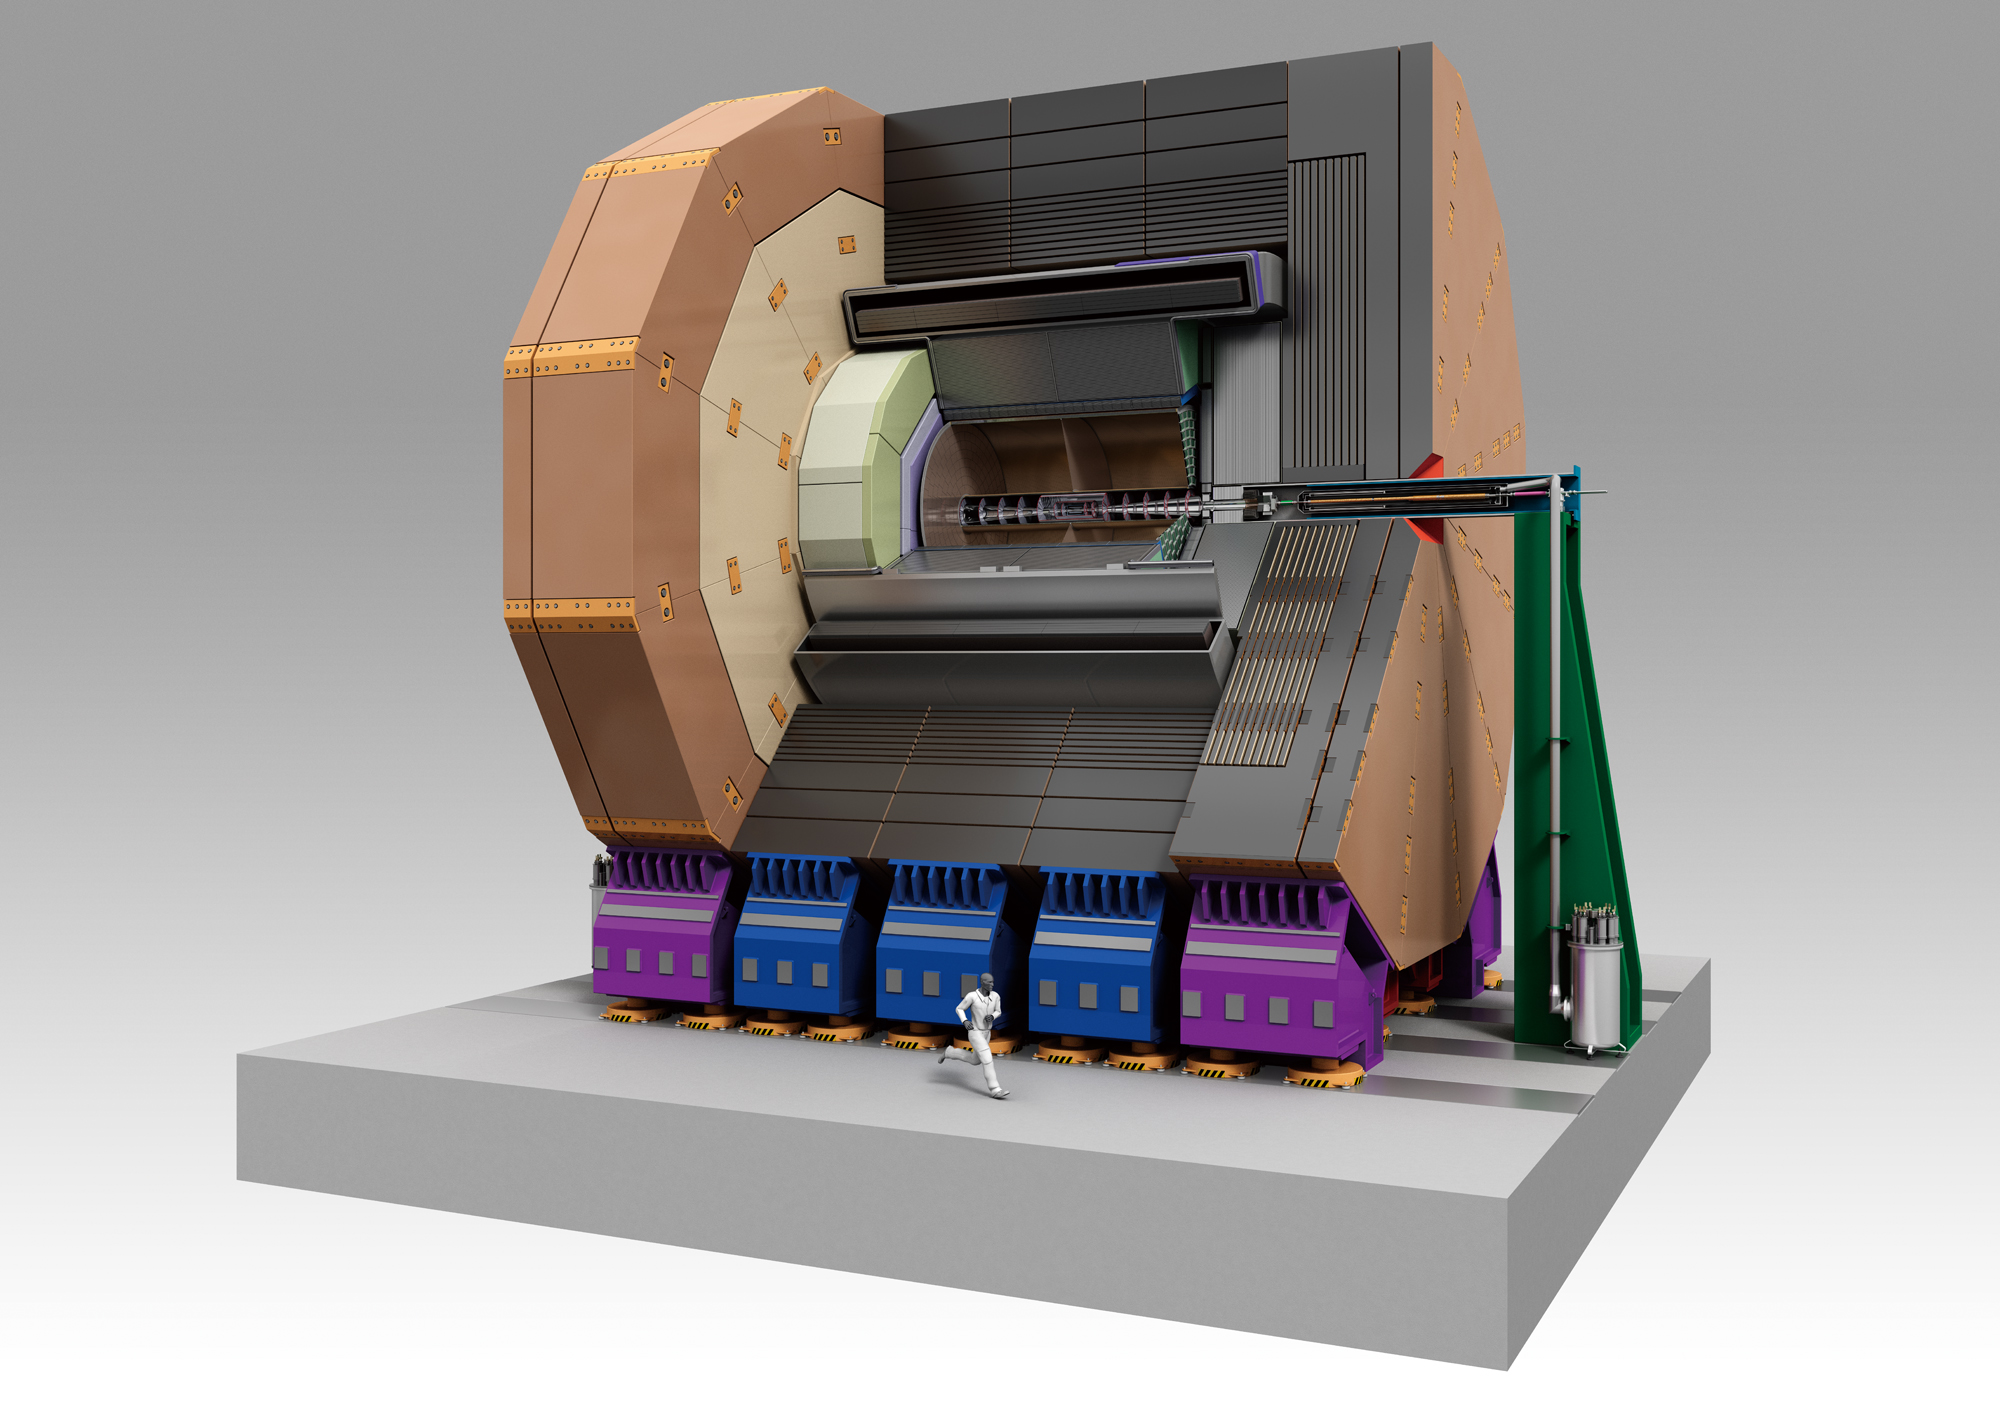
\includegraphics[width = 0.4\textwidth]{Pictures/ILD.jpg}
    \caption{Schéma de l'ILD, un des deux détecteurs prévus à l'ILC.}
    \label{fig:ILD}
  \end{figure}
 
  Un nouveau grand projet en physique des hautes énergies est à l'étude : l'International Linear Collider (ILC). 
  Ce collisionneur linéaire de 31 kilomètres de long permettra la collision d'électrons et de positrons à une échelle d'énergie comprise entre 250 GeV et 500 GeV et ultérieurement 1 TeV, pour des polarisations différentes.
  %En effet, les électrons et positrons sont des particules fondamentales qui permettent de contrôler précisément l'énergie de collision et de sélectionner les processus à étudier grâce à la polarisation de ces dites particules.
  Grâce à l'étude des collisions electrons/positrons reposant sur l'identification complète des processus quantiques de chaque évènement, ce nouveau collisionneur devrait permettre de mieux caractériser les particules déjà connues, comme le boson de Higgs grâce à son couplage avec les fermions, mais aussi d'étudier la matière noire.
 % Il devrait permettre de mieux caractériser les particules déjà connues, comme le boson de Higgs grâce à son couplage avec les fermions, mais aussi d'étudier la matière noire. 
  Pour cela la partie centrale du détecteur, dédiée à la reconstruction des chaînes de désintégration survenues avant la première couche instrumentée, doit avoir à la fois une excellente résolution spatiale et un budget de matière ($X_0$) ne dépassant pas quelques millièmes de la longueur de radiation. 
  Ce sous-détecteur, appelé détecteur de vertex, doit être optimisé afin de permettre la trajectométrie dans un milieu hautement dense en particules et de différencier la trajectoire des quarks $b$ et $c$.

  La collaboration PLUME, qui implique l'IPHC de Strasbourg, le DESY à Hambourg et l'université de Bristol, met en place les outils permettant de surmonter ces défis grâce à une conception innovante d'échelles de trajectométrie double face pixelisée, appelée PLUME\footnote{\textbf{P}ixelated \textbf{L}adder with \textbf{U}ltra low \textbf{M}aterial \textbf{E}mbeded}\cite{PLUME}. 
  Ce type d'objet est équipé de six capteurs à pixels CMOS ultra fins (amincis à $\sim 50 \text{ }\mu\text{m}$), alignés l'un à côté de l'autre, sur chaque face d'un support mécanique très léger et tente d'atteindre un record au niveau du budget de matière en se rapprochant de 0.3\% de $X_0$.
  La figure~\ref{fig:PLUME} est un schéma représentant le principe d'une échelle double face développée par la collaboration.
  Pour chaque trajectoire, deux positions seront mesurées, une par face. 
  Elles permettront d'évaluer le point d'intersection de la particule avec le détecteur, mais aussi son mouvement et son origine. 
  Si les outils permettant cette double mesure sont maitrisés et optimisés, cela augmentera considérablement les capacités de trajectométrie de ce type d'instrument.

  \begin{figure}
    \centering
    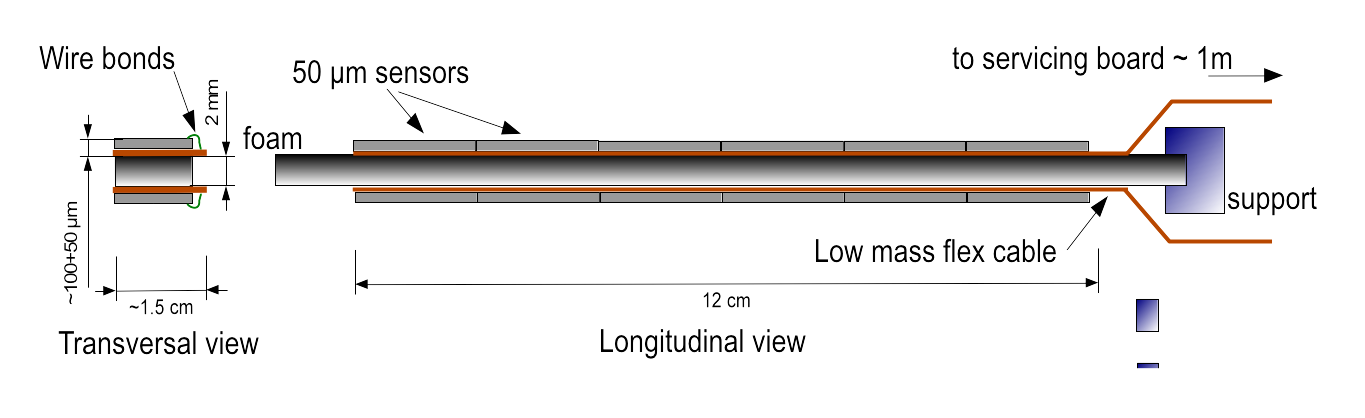
\includegraphics[width = 0.8\textwidth]{Pictures/plume_finalGoal.png}
    \caption{Schéma du principe final de l'échelle PLUME.}
    \label{fig:PLUME}
  \end{figure}

  Ma thèse vise à participer à la construction de la seconde génération de détecteurs de PLUME et à caractériser leurs performances.

  \section{Étude (simpliste) de la désintégration du boson de Higgs}

  Afin de comprendre les paramètres du système de détection, j'ai démarré une analyse de physique concernant la désintégration du boson de Higgs en deux paires de quarks charmé et anti-charmé à une énergie de centre de masse de 350 GeV à l'ILC, avec des données simulées par méthode Monte Carlo.

    \begin{figure}  
        \centering
        \begin{subfigure}[t]{0.3\textwidth}
            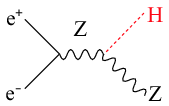
\includegraphics[width = 0.8\textwidth]{Pictures/Chapter_Theory_figs_ZHdiagram.png}
            \caption{Higgs-Strahlung.}
            \label{fig:higgsStrahlung}
        \end{subfigure}
        ~%\qquad
         %add desired spacing between images, e. g. ~, \quad, \qquad, \hfill etc. 
          %(or a blank line to force the subfigure onto a new line)
        \begin{subfigure}[t]{0.3\textwidth}
            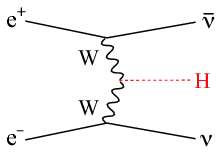
\includegraphics[width = 0.8\textwidth]{Pictures/Chapter_Theory_figs_nunuHdiagram.png}
            \caption{Fusion de bosons W.}
            \label{fig:WW-fusion}
        \end{subfigure}
        ~%\qquad
         %add desired spacing between images, e. g. ~, \quad, \qquad, \hfill etc. 
          %(or a blank line to force the subfigure onto a new line)
        \begin{subfigure}[t]{0.3\textwidth}
            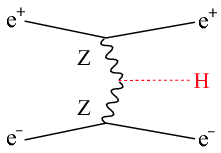
\includegraphics[width = 0.8\textwidth]{Pictures/HiggsProd_eeH.png}
            \caption{Fusion de bosons Z.}
            \label{fig:ZZ-fusion}
        \end{subfigure}
        \caption{Diagrammes de Feynman des principaux processsus de production du boson de Higgs à l'ILC\cite{Asner2013}\cite{tian}.}
        \label{fig:higgsProduction}
    \end{figure}    

  Contrairement aux canaux de production du boson de Higgs disponible au LHC, l'ILC est capable de produire directement le Higgs, soit par Higgs-strahlung (voir figure~\ref{fig:higgsStrahlung}), soit par la fusion de bosons W (voir figure~\ref{fig:WW-fusion}) ou alors par la fusion de bosons Z (voir figure~\ref{fig:ZZ-fusion}).
  Néanmoins, à 350 GeV, seulement le Higgs-strahlung et la fusion WW sont observables.
  Je me suis tout particulièrement intéressé à l'état final comportant un boson de Higgs et deux neutrinos.
  %L'état final qui m'a intéressé est celui où le Higgs et deux neutrinos sont produits, soit par Higgs-strahlung (voir figure~\ref{fig:higgsStrahlung}), soit par fusion de bosons W (voir figure~\ref{fig:WW-fusion}).
  Ces canaux de production permettent une observation particulièrement précise des propriétés du boson de Higgs. 
  En effet, les particules détectées dans l'état final proviennent uniquement de la désintégration du boson de Higgs. 
  Par ailleurs, la production via Higgs-strahlung autorise une étude du boson de Higgs sans considérations des produits de désintégrations, en étudiant simplement la masse de recule.
  
  L'étude m'a d'abord permis de comprendre l'avantage de la polarisation des électrons et positrons sur le canal de physique que l'on souhaite étudier.
  Par exemple, la contribution de la fusion de bosons W est atténuée lorsque les électrons sont droits et les positrons gauches.
  Cependant, le signal étudié est noyé dans un bruit de fond généré pas d'autres processus.
  Deux bruits de fonds sont considérés, ceux menant à un état final identique à notre signal, ou alors ceux produisant un réponse dans le détecteur similaire à celle du signal.
  Afin de différencier le signal du bruit, certains critères doivent être définis.
  Tout d'abord, nous nous attendons à observer deux jets provenant de la désintégration du boson de Higgs. 
  Ainsi, tous les évènements ne contenant qu'un lepton isolé ne sont pas pris en compte.
  Puis, une sélection sur l'impulsion transverse visible est effectuée afin de réduire l'impact des hadrons produits par interaction $\gamma\gamma$.
  Ensuite, les évènements sont sélectionnés par rapport à l'hypothèse sur la structure de notre signal.
  Par exemple, la masse visible doit correspondre à la signature du boson de Higgs, qui est de 125 GeV.
  La résolution de ce paramètre dépend de la résolution en énergie des jets. 
  D'autres paramètres sont utilisés comme par exemple l'angle entre les deux jets.
 % D'autres paramètres sont utilisés comme par exemple l'impulsion transverse visible, la masse visible ou encore l'angle entre les deux jets.
  Ainsi, il est possible d'améliorer la significance (ratio du signal sur la raciné carré du signal et du bruit) d'un facteur 10 après sept sélections différentes.
  Bien que le bruit soit diminué d'un facteur de plus de 200, le signal intéressant a lui aussi été diminué d'un facteur 1.4.

  La suite de ce travail consiste a étudier la capacité d'identifier les quarks charmés pour différentes géométries de détecteur de vertex. 
  Malheureusement, dû au temps qui m'a été imparti pour effectuer cette thèse, je n'ai pu effectuer cette étude.

  \section{Préparation d'une campagne de tests sous faisceaux}

    Comme décrit en introduction, l'objectif de la collaboration PLUME est d'atteindre un budget de matière se rapprochant de 0.3 \% de $X_0$ pour une résolution spatiale meilleure que 4 microns.
  La structure mécanique est validée grâce à l'utilisation de MIMOSA-26, des détecteurs monolithiques complexes qui ont une résolution spatiale de $< 4$ $\mu$m.
  Le traitement des données est directement intégré dans les photocites qui collectent les charges. 
  Il permet de numériser directement le signal, grâce à des discriminateurs et de réduire la bande-passante de transmission des données par le biais d'un système de suppression de zéro (ne prend pas en compte les zéros envoyés par les pixels, qui ne représentent pas un signal physique intéressant).
  Cette méthode permet d'enregistrer les informations individuelles de plus de un million d'impacts/cm$^2$/s sur un capteur contenant plus de 500000 pixels sur une surface de 2 cm$^2$.
  
   \subsection{Validation en laboratoire des échelles PLUME}

  Les échelles PLUME sont les premiers prototypes double faces associant un budget de matière se rapprochant de 0.3 \% de $X_0$ et des pistes métallisées adaptées à la surface de détection de $1 \times 12 \text{cm}^2$, afin de réduire les zones mortes du détecteurs. 
  Chaque module doit être validé en laboratoire afin de s'assurer que l'assemblage n'altère pas les capteurs utilisés.
  Après une inspection visuelle afin de contrôler l'alignement de chaque capteur l'un par rapport à l'autre et qu'aucun d'eux, ni aucune connexion n'ait été endommagé pendant l'assemblage, chaque échelle est testée électriquement.
  La consommation des capteurs, le contrôle JTAG ainsi que la présence de pixels morts sont vérifiés, pour ensuite évaluer les seuils des comparateurs qui vont permettre de discriminer le signal du bruit.
  Leur point de fonctionnement optimal, leur bruit et piédestal sont obtenus grâce à une courbe de transfert qui représente la réponse des comparateurs à différents seuils et permet de définir un seuil où le bruit du capteur est supprimé sans en altérer ces capacités de détection.
  Ensuite, les propriétés de détection de ces capteurs sont contrôlés grâce à une analyse qui permet de déterminer le taux de fantôme de chaque capteur et de vérifier qu'ils détectent correctement une source radioactive.
  
    \subsection{Étude de la déformation des échelles lors d'une campagne de faisceau test}

  Actuellement, différentes versions des échelles PLUME existent : celles dont le budget de matière est de 0.6 \% de $X_0$ utilisant uniquement des pistes métallisées en cuivre; deux nouveaux prototypes, l'un utilisant des pistes métallisées en cuivre et l'autre en aluminium et dont les zones mortes de détection ont été réduites et la densité de la mousse mécanique a été diminuée de moitié.
  Bien que différentes versions existent, seuls les modules atteignant un budget de matière de 0.6 \% de $X_0$ ont été étudiés lors de deux campagnes en faisceau test, l'une réalisée par la collaboration en 2011 au CERN et l'autre que j'ai mené en avril 2016 au DESY.
  Les résultats de la première campagne ont permis à la collaboration de mettre en avant les avantages d'une double mesure. 
  De ces résultats, je me suis intéressé à l'étude des déformations mécaniques de nos échelles et leur impact sur les résultats d'analyse.
  En effet, lorsque l'échelle est inclinée dans une direction et que le faisceau ne la touche plus en incidence normale, la résolution spatiale se dégrade dans des proportions inattendues.
  Ce comportement est dû aux contraintes mécaniques qui induisent des déformations permanentes de quelques dizaines de micromètres de la surface ne pouvant être contrôlées lors de l'assemblage.
  Apprendre à quantifier ces déformations et les prendre en compte pendant notre analyse est essentiel pour valider nos prototypes.
  Les capteurs sont modélisés par une surface parfaitement plane.
  Or, la position de ces plans en trois dimensions est différente puisque ceux-ci peuvent être plus ou moins déformés.
  Ainsi comme il a été observé, la distribution du résidu, ou distance entre la position du pixel touché et de la trace extrapolée, devient plus importante lorsque l'angle d'incidence n'est plus normal à la surface du détecteur.
  Il faut donc prendre en compte cette déformation dans notre analyse afin de recalculer la position exacte de chaque pixel en 3 dimensions et l'extrapolation exacte sur le plan de la trajectoire. 
  Grâce à une première étude réalisée par un doctorant du groupe PICSEL et un article de la collaboration CMS sur l'alignement du trajectomètre\cite{Chatrchyan:2009sr}, il m'a été possible de mettre en place un algorithme permettant de déterminer la forme de notre capteur à l'aide de polynômes de Legendre. 
  En prenant en compte l'angle d'incidence des particules, la résolution spatiale est améliorée. 
  Par exemple, l'analyse d'une acquisition où le module PLUME est incliné de 28\degre, a mis en évidence une déformation en corrélant le résidu à la position de l'impact sur la matrice de détection, par rapport à une acquisition où le plan est en incidence normale.
  En ajustant la figure~\ref{fig:deformation} (celle du milieu) par un polynôme de Legendre, les coefficients obtenus permettent de paramétrer la surface du capteur et ainsi de minimiser le résidu, comme montré sur la figure~\ref{fig:correction}. 
  La déviation standard de les distribution des résidus, qui définit la résolution spatiale, passe de 9.8 $\mu m$ à 5.3 $\mu m$, sans prendre en compte la résolution du télescope qui n'est pas dans une configuration optimale.


    \begin{figure}  
        \centering
        \begin{subfigure}[t]{0.4\textwidth}
            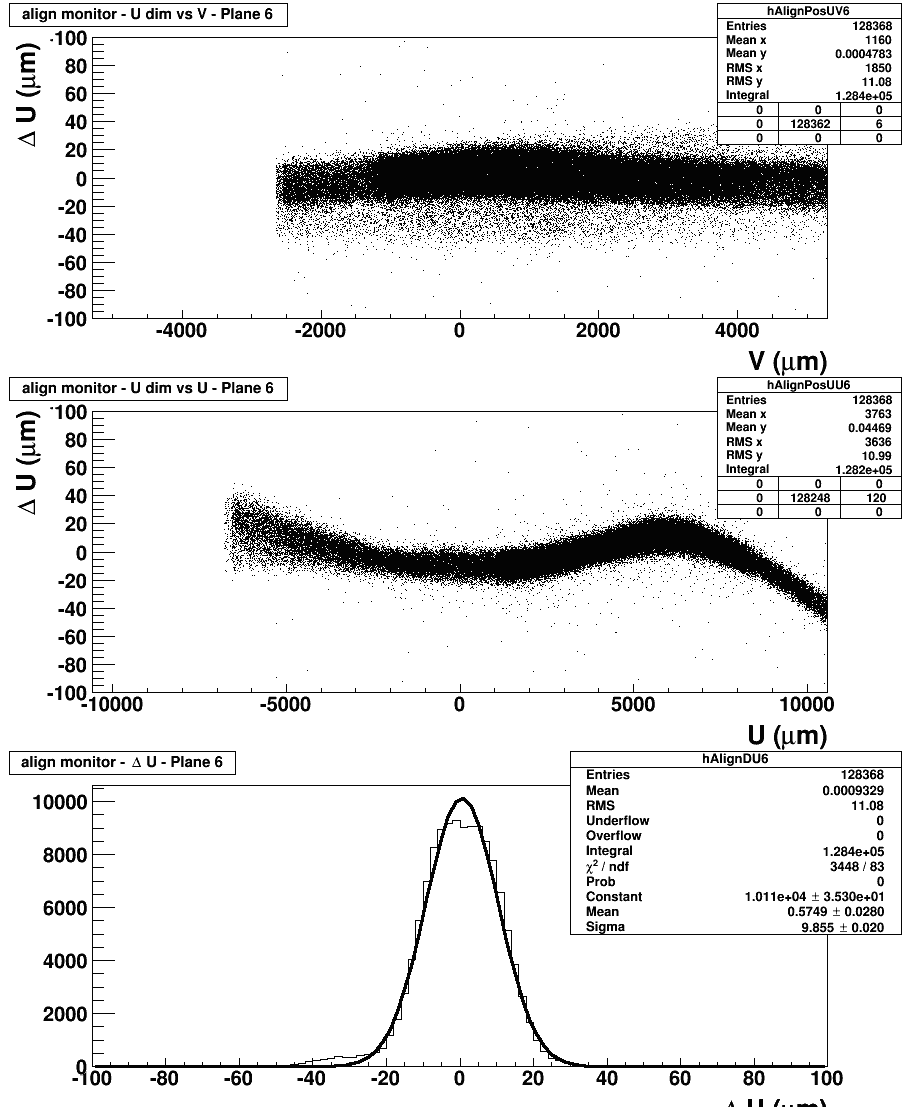
\includegraphics[width = 0.8\textwidth]{Pictures/RsAlign_226021_pl6_deformed2.png}
            \caption{Avant la prise en compte des déviations. }
            \label{fig:deformation}
        \end{subfigure}
        ~%\qquad
         %add desired spacing between images, e. g. ~, \quad, \qquad, \hfill etc. 
          %(or a blank line to force the subfigure onto a new line)
        \begin{subfigure}[t]{0.4\textwidth}
            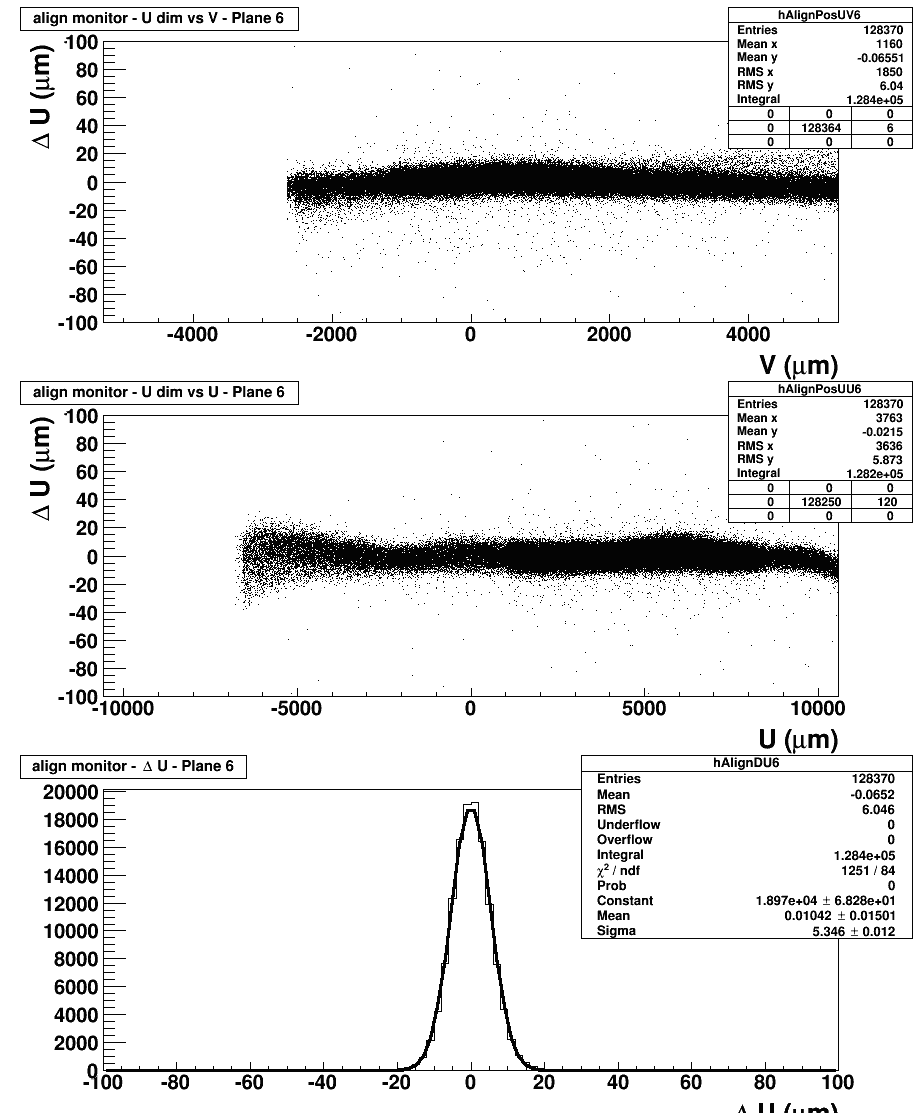
\includegraphics[width = 0.8\textwidth]{Pictures/RsAlign_226021_pl6_corrected2.png}
            \caption{Après la prise en compte des déviations.}
            \label{fig:correction}
        \end{subfigure}
        \caption{Graphiques représentant la distance point d'impat/trace sur la direction horizontale en fonction de la position du point d'impact dans la direction verticale (haut), la distance point d'impact/trace dans la direction horizontale en fonction de la position du point d'impact dans la même direction (milieu) ainsi que la distribution de la distance du point d'impact par rapport à la position de la trace (bas). La correction permet d'atteindre une résolution de 5.3 $\mu$m au lieu de 9.8 $\mu$m.}
        \label{fig:defCor}
    \end{figure}    

    \subsection{Estimation du budget de matière avec des électrons de basse énergie}

  Nos échelles doivent avoir des performances similaires à basse énergie à celles obtenus lors du précédent faisceau test.
  En effet, le détecteur de vertex doit être capable de mesurer tant les particules qui ont une grande impulsion, des particules qui ont une faible impulsion et qui ne pourront être détectées par les autres parties de ce détecteur.
  C'est pourquoi, j'ai préparé et effectué une deuxième campagne de faisceau test avec des électrons de quelques GeV au DESY en avril 2016.
  Avant d'effectuer cette expérience, il m'a fallu m'assurer de l'intégration de notre détecteur au sein du système d'acquisition EUDAQ fourni par le DESY. 
  Un outil de simulation estimant la résolution spatiale en fonctions de différentes géométrie de télescope m'a permis de définir une géométrie optimale pour étudier à la fois les caractéristiques attendues de l'échelle, mais aussi de pouvoir déterminer son budget de matière et le comparer aux attentes théoriques.
  Comme la technologie des capteurs utilisés pour le télescope et PLUME sont les mêmes, le système d'acquisition a été simplifié : deux plans de télescopes sont positionnés de part et d'autres du détecteur afin de mesurer la trajectoire des particules. 
  Des mesures de plusieurs heures ont permis de vérifier la stabilité du système d'acquisition. 
  En même temps, un support rotatif a été construit afin de maintenir l'échelle à la position verticale et de permettre une prise de données pour des angles variants de 0\degre à 60\degre.
  La figure~\ref{fig:testBeam} a été prise durant la campagne de faisceau test et montre le positionnement de l'échelle PLUME, située au centre entre les quatre plans de référence.
  L'analyse est actuellement en cours et tente de mesurer pour la première fois le budget de matière de nos échelles dans des conditions réelles, ainsi que de confirmer l'avantage d'une mesure de la position du pixel touché sur chaque face.
  En effet, la combinaison des deux informations permet d'améliorer la résolution spatiale obtenue tout en donnant l'accès à une nouvelle information, la résolution angulaire de l'échelle.

  \begin{figure}
    \centering
    \includegraphics[width=0.5\textwidth]{Pictures/testBeam.jpg}
    \caption{Photo prise pendant la campagne de faisceau test au DESY. L'échelle PLUME est montée sur un support rotatif et est située entre les quatre plans de référence.}
    \label{fig:testBeam}
  \end{figure}

  \section{Conclusions}
 
  Au cours de mon travail de thèse, j'ai pu étudier l'intérêt d'un collisionneur linéaire électrons/positrons afin de réaliser des mesures précises des propriétés du boson de Higgs.
  Je me suis tout particulièrement intéressé à un canal de désintégration inaccessible au LHC où l'état final comporte le boson de Higgs ainsi que deux neutrinos. 
  Les différents critères permettant de différencier le signal étudié du bruit ont été étudiés grâce à des sélections sur la région d'intérêt.
  Malheureusement, le temps qui m'a été imparti pour réaliser mes travaux ne m'a pas permis d'étudier les performances d'identification des quarks charmés pour différentes géométries de détecteur de vertex.

  Ma recherche c'est principalement concentrée sur de l'étude et de la validation des premiers concepts d'échelles de détections double faces atteignant un budget de matière de seulement 0.3 \% $X_0$.
  Un banc de validation a été mis en place au DESY et a permis de vérifier que les performances des capteurs utilisés ne sont pas impactées par la structure unique de ces échelles.
  Par ailleurs, les résultats de la campagne en faisceau test effectuée au CERN en 2011 ont permis de mettre en évidence l'impact de la déformation des capteurs sur la résolution spatiale de notre échelle lorsque celle-ci ne se trouve plus en incidence normale.
  L'algorithme développé qui utilise des polynômes de Legendre pour extrapoler la position des capteurs en trois dimensions a permis de réduire l'impact des déformations sur les résultats d'analyse en faisceau test.
  Bien que les résultats soient encourageants, l'algorithme peut-être amélioré en utilisant une méthode itérative afin de déterminer plus précisément la position de l'impact sur le capteur.
  
  Enfin, grâce au faisceau délivré par le DESY, ainsi que différents logiciels d'analyse ont permis à la collaboration de réaliser pour la première fois la mesure du budget de matière de nos échelles.
  Les premiers résultats devraient être obtenus afin la soumission du manuscrit et présentés lors de la soutenance de thèse.

  Le travail effectué au cours de ces trois années sont prometteurs pour une utilisation des échelles PLUMES dans le cadre de l'ILC.
  D'autres applications sont par ailleurs possibles, comme son utilisation pour l'estimation des conditions de bruit de fond machine dans l'expérience BEAST, juste avant le démarrage de Belle-II.

 
  \section*{Publications et conférences}

  Conférences :
  \begin{itemize}
    \item \textit{3$^{rd}$ Beam Telescopes and Test Beams Workshop}, Janvier 2015, DESY - Hambourg (Allemagne); présentation orale\\
    "Observing and correcting the surface deformation of light pixelated detection surface"
    \item \textit{2015 International Workshop on Future Linear Colliders (LCWS15)},Novembre 2015,  Whistler (Canada); présentation orale\\
    "Double-sided pixelated layers studies from the PLUME collaboration"
  \end{itemize}
  Publication :
  
  B. Boitrelle, J. Baudot, G. Claus, O. Clausse, L. Cousin, R. Gauld, M. Goffe, J. Goldsteind, I.M. Gregor, M. Imhoff, U. Koetz, R. Maria, A. Nomerotski, R. Page, M. Szelezniak and M. Winter "The PLUME performance evaluation" (en préparation)

  \section*{Formations}
 
  \begin{itemize}
    \item Linear Collider Physics School\footnote{https://indico.desy.de/conferenceDisplay.py?confId=7513} au DESY à Hambourg du 7 au 9 octobre 2013
    \item 7$^{th}$ Detector Workshop of the Terascale Alliance\footnote{https://indico.desy.de/conferenceDisplay.py?confId=9389} à Göttingen du 3 au 5 mars 2014
    \item Introduction to Terascale 2014\footnote{https://indico.desy.de/conferenceDisplay.py?confId=9263} au DESY à Hambourg du 17 au 21 mars 2014
    \item Linear Collider School 2014\footnote{https://indico.desy.de/conferenceDisplay.py?confId=9329} à Frauenchiemsee du 11 au 15 août 2014
    \item Introduction school on thermal and mechanical simulations based on finite-element calculations à Berlin du 2 au 4 Mars 2015
    \item Cours d'allemand au DESY, septembre 2013 à février 2014 (3 heures par semaine)
    \item Cours d'allemand avec la PIER school depuis avril 2015 (1 heure 30 par semaine)
  \end{itemize}

  \bibliographystyle{plain}
	\bibliography{Bibliography/biblio}
 \end{document}
